% !TeX recipe = Tectonic
% CV - Marko Rosic - tailored for Almedia, Head of Product Design
% Compile with: cd applications/almedia && tectonic Marko_Rosic_CV.tex
\documentclass[a4paper,9.5pt]{article}

% ── Font ──────────────────────────────────────────────────────────────
\usepackage{fontspec}
\setmainfont{Fira Sans}[
  BoldFont       = {Fira Sans Bold},
  ItalicFont     = {Fira Sans Italic},
  BoldItalicFont = {Fira Sans Bold Italic}
]
\newfontfamily\symfont{Zapf Dingbats}

% ── Layout ────────────────────────────────────────────────────────────
\usepackage[a4paper, top=1.5cm, bottom=1.4cm, left=1.8cm, right=1.8cm]{geometry}
\usepackage{microtype}
\usepackage{needspace}

% ── Colors ────────────────────────────────────────────────────────────
\usepackage{xcolor}
\definecolor{darktext}{HTML}{111111}
\definecolor{midgray}{HTML}{555555}
\definecolor{lightgray}{HTML}{999999}
\definecolor{hairline}{HTML}{BBBBBB}

% ── Links ─────────────────────────────────────────────────────────────
\usepackage[hidelinks]{hyperref}
\urlstyle{same}
\usepackage[normalem]{ulem}

% ── Lists ─────────────────────────────────────────────────────────────
\usepackage{enumitem}

% ── Tables ────────────────────────────────────────────────────────────
\usepackage{array}

% ── TikZ ──────────────────────────────────────────────────────────────
\usepackage{tikz}
\usetikzlibrary{calc}

% ── Section headings ──────────────────────────────────────────────────
\usepackage{titlesec}
\titleformat{\section}
  {\normalfont\small\bfseries}
  {}{0em}{\MakeUppercase}
  [\vspace{3pt}{\color{darktext}\hrule height 0.4pt}]
\titlespacing*{\section}{0pt}{22pt}{12pt}

% ── Page style ────────────────────────────────────────────────────────
\pagestyle{empty}
\setlength{\parindent}{0pt}
\setlength{\parskip}{0pt}

% ── Column dimensions ─────────────────────────────────────────────────
\newlength{\cvdatecol}  \setlength{\cvdatecol}{2.5cm}
\newlength{\cvsymcol}   \setlength{\cvsymcol}{1cm}
\newlength{\cvcontcol}  \setlength{\cvcontcol}{\dimexpr\textwidth-\cvdatecol-\cvsymcol\relax}

% ── Symbol counter ────────────────────────────────────────────────────
\newcounter{cvsymn}
\newif\ifcvfirst\cvfirsttrue

% ── TikZ asterisk with named remember-picture node ───────────────────
\newcommand{\cvastsym}{%
  \begin{tikzpicture}[remember picture, baseline=(sym-\thecvsymn.base)]
    \node[inner sep=0pt, outer sep=0pt, text=darktext, font=\normalsize\symfont] (sym-\thecvsymn) {✱};
  \end{tikzpicture}%
}

% ── Portfolio button ──────────────────────────────────────────────────
\newcommand{\portfoliobutton}{%
  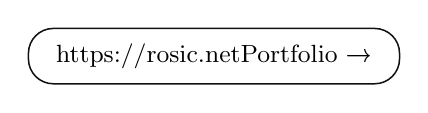
\begin{tikzpicture}[baseline=(btn.base)]
    \node[draw=darktext, rounded corners=9pt,
          inner xsep=10pt, inner ysep=5.5pt,
          line width=0.55pt, font=\small,
          outer sep=0pt] (btn)
      {\href{https://rosic.net}{Portfolio~→}};
  \end{tikzpicture}%
}

% ── Connector: hairline from prev asterisk to current, same page only ─
\newdimen\cvyprev
\newdimen\cvycurr
\newcommand{\cvdrawconnect}{%
  \edef\prevn{\the\numexpr\value{cvsymn}-1\relax}%
  \begin{tikzpicture}[overlay, remember picture]
    \coordinate (cvprev) at (sym-\prevn.center);
    \coordinate (cvcurr) at (sym-\thecvsymn.center);
    \pgfextracty{\cvyprev}{\pgfpointanchor{cvprev}{center}}%
    \pgfextracty{\cvycurr}{\pgfpointanchor{cvcurr}{center}}%
    \ifdim\cvyprev>\cvycurr%
      \draw[line width=0.35pt, color=hairline]
        ($(sym-\prevn)+(0,-4.5pt)$) -- ($(sym-\thecvsymn)+(0,4.5pt)$);%
    \fi%
  \end{tikzpicture}%
}

% ── Entry without company note ────────────────────────────────────────
\newcommand{\cventry}[3]{%
  \stepcounter{cvsymn}%
  \par\vspace{13pt}%
  \noindent%
  \makebox[\cvdatecol][r]{\small\bfseries\color{midgray}#1}%
  \makebox[\cvsymcol][c]{\cvastsym}%
  \parbox[t]{\cvcontcol}{%
    {\bfseries #2}\\[2.5pt]
    {\small#3}%
  }%
  \ifcvfirst\cvfirstfalse\else\cvdrawconnect\fi%
  \par%
}

% ── Entry with italic company context line ────────────────────────────
\newcommand{\cventrynote}[4]{%
  \stepcounter{cvsymn}%
  \par\vspace{13pt}%
  \noindent%
  \makebox[\cvdatecol][r]{\small\bfseries\color{midgray}#1}%
  \makebox[\cvsymcol][c]{\cvastsym}%
  \parbox[t]{\cvcontcol}{%
    {\bfseries #2}\\[2.5pt]
    {\small#3}\\[2.5pt]
    {\footnotesize\itshape\color{lightgray}#4}%
  }%
  \ifcvfirst\cvfirstfalse\else\cvdrawconnect\fi%
  \par%
}

% ── Bullet list ───────────────────────────────────────────────────────
\newenvironment{cvitems}{%
  \vspace{1pt}%
  \begin{itemize}[
    leftmargin = \dimexpr\cvdatecol+\cvsymcol+0.55em\relax,
    label      = {•},
    topsep     = 4pt,
    itemsep    = 3pt,
    parsep     = 0pt,
    partopsep  = 0pt
  ]\small\interlinepenalty=10000%
}{\end{itemize}}

% ── Skill block ───────────────────────────────────────────────────────
\newcommand{\skillblock}[2]{%
  {\small\bfseries #1}\newline%
  {\small\color{midgray}#2}%
}

% ══════════════════════════════════════════════════════════════════════
\begin{document}
% ══════════════════════════════════════════════════════════════════════

% ── HEADER ────────────────────────────────────────────────────────────
\vspace*{-0.3cm}
\noindent{\fontsize{30}{36}\selectfont\bfseries Marko Rosić}%
\hfill\makebox[0pt][r]{\portfoliobutton\hspace{2pt}}
\par\vspace{3pt}
{\small\color{midgray}%
  Cara Du\v{s}ana 118, Belgrade, Serbia~\textbar~%
  +381 60 585 44 55~\textbar~%
  \href{mailto:marko@rosic.net}{\uline{marko@rosic.net}}~\textbar~%
  \href{https://rosic.net}{\uline{rosic.net}}%
}

% ── SUMMARY ───────────────────────────────────────────────────────────
\section{Summary}

{\small Head of Design with 15+ years building consumer products and
the design infrastructure behind them. I own end-to-end product
experience, build and lead small teams that do quality work without
hand-holding, and connect design systems to real business outcomes.
I work hands-on: I prototype, build Figma plugins, and use AI including
Claude Code to ship faster. I cut development time by 30\% and
time-to-market by 25\% through design systems and better
design-engineering collaboration at the companies I've led design for.}

% ── EXPERIENCE ────────────────────────────────────────────────────────
\section{Experience}

\cventry{5/2025\,--\,Present}{Design Leadership Consultant}{%
  Beyond Clicks Studio (Independent) \textbar{} Belgrade, Serbia (Remote)}
\begin{cvitems}
  \item Led design end to end as Head of Design for an international
        consumer platform: retention and onboarding flows, conversion
        optimisation, progressive filter architecture, and high-fidelity
        transactional email templates
  \item Architected a multi-brand design system from scratch: token
        architecture, Figma variables pipeline connecting directly to
        theme tokens, and a full component library
  \item Redesigned key conversion surfaces, improving revenue card
        performance and reducing drop-off across transactional flows
  \item Built AI-orchestrated workflows using Claude Code to ship UX and
        internal tooling faster; built Figma plugins to automate
        production tasks and reduce design-engineering drift
  \item Managed and mentored a graphic designer, delegating routine
        production to focus on product strategy and core UX
\end{cvitems}

\cventrynote{7/2024\,--\,5/2025}{Head of UX/UI}{%
  Gentoo Media \textbar{} Belgrade, Serbia}{%
  Established following GiG Media's acquisition of Catena Media and
  subsequent spin-off of its media division.}
\begin{cvitems}
  \item Built a company-wide design system across multi-brand consumer
        products, setting token architecture, component conventions, and
        handoff standards
  \item Led a design team of seven including two team leads, owning their
        direction, growth, and performance
  \item Cut feature time-to-market by 25\% by changing how design and
        engineering worked together
  \item Used analytics and user feedback to drive continuous product
        improvement
\end{cvitems}

\cventry{5/2021\,--\,7/2024}{Lead UX/UI Designer}{%
  Catena Media (acquired by GiG Media in 2023) \textbar{} Belgrade, Serbia}
\begin{cvitems}
  \item Directed end-to-end UX for high-traffic, multi-market consumer
        web products serving millions of users per month across 10+
        websites
  \item Built a design system for the flagship product that cut
        development time by 30\%
  \item Ran stakeholder workshops to align design decisions with business
        goals; mentored junior designers
\end{cvitems}

\cventry{10/2018\,--\,5/2021}{Senior UX/UI Designer}{%
  Catena Media \textbar{} Belgrade, Serbia}
\begin{cvitems}
  \item Led the flagship product redesign: mobile traffic up 20\%, user
        retention up 15\%
  \item Brought user research and A/B testing into the product process,
        moving the team to evidence-based decisions
  \item Drove the team's migration from Sketch to Figma
\end{cvitems}

\needspace{5\baselineskip}
\cventry{12/2013\,--\,10/2018}{Interaction Designer}{%
  Smith Micro Software, Inc \textbar{} Belgrade, Serbia}
\begin{cvitems}
  \item Designed UX for carrier-branded Android apps shipped with Sprint
        and T-Mobile: Visual Voicemail, messaging, and device companion
        tools
  \item Designed backend tooling for device management and an IoT
        location-based notification system
\end{cvitems}

\cventry{2009\,--\,2013}{UI Designer}{%
  MySkin, Youngculture \textbar{} Belgrade, Serbia}
\begin{cvitems}
  \item Designed digital products and interfaces across client projects
\end{cvitems}

\cventry{2005\,--\,2008}{Co-founder \& CEO}{%
  Mainstream d.o.o. \textbar{} Belgrade, Serbia}
\begin{cvitems}
  \item Co-founded a dial-up ISP; led operations, finance, and product
        design during the founding phase
\end{cvitems}

% ── SKILLS ────────────────────────────────────────────────────────────
\section{Skills}

\vspace{2pt}
\noindent
\begin{minipage}[t]{0.475\textwidth}
  \skillblock{Product Design \& UX}{%
    End-to-end product UX, consumer
    product design, conversion optimisation,
    user research \& usability testing,
    A/B testing, Figma, Axure RP}

  \vspace{12pt}
  \skillblock{Data \& Analytics}{%
    Google Analytics, VWO, HotJar,
    UXtweak, Optimal Workshop}
\end{minipage}%
\hspace{0.05\textwidth}%
\begin{minipage}[t]{0.475\textwidth}
  \skillblock{Leadership \& Design Systems}{%
    Design team management \& mentoring,
    Design systems (token architecture,
    component libraries), DesignOps,
    Roadmap \& stakeholder management,
    Jira, Asana, Linear, Notion}

  \vspace{12pt}
  \skillblock{Technical}{%
    HTML/CSS, JavaScript, PHP,
    Figma plugin development,
    AI-orchestrated delivery (Claude Code)}
\end{minipage}

% ── LANGUAGES ─────────────────────────────────────────────────────────
\section{Languages}

\begin{itemize}[leftmargin=1.2em, label={•},
    topsep=0pt, itemsep=2pt, parsep=0pt]
  \item {\small\textbf{English:} Fluent (Business Proficiency)}
  \item {\small\textbf{French:} Intermediate}
  \item {\small\textbf{Serbian:} Native}
\end{itemize}

% ── EDUCATION ─────────────────────────────────────────────────────────
\section{Education}

\noindent{\small\bfseries Bachelor of Economics}\\[1pt]
{\small\color{midgray}Faculty for Business Studies,
Megatrend University, Belgrade \hfill 2002\,--\,2008}

\vspace{6pt}

\noindent{\small\bfseries Industrial Design Technician}\\[1pt]
{\small\color{midgray}School for Design, Belgrade
\hfill 1995\,--\,1999}

% ── AWARDS ────────────────────────────────────────────────────────────
\needspace{4\baselineskip}
\section{Awards}

{\small\textbf{Best of Swiss Apps — Gold, Entertainment} \hfill 2013\\
\color{midgray}Swisscom TV Android tablet app}

\end{document}
